\documentclass[11pt]{article}
%%%%%%%%% options for the file macros.tex

\def\showauthornotes{1}
\def\showkeys{0}
\def\showdraftbox{0}
% \allowdisplaybreaks[1]

%% Shamelessly adapted from a scribe template by Sanjeev Arora

%%%%%%%%%%%%%% Packages
% \usepackage[active,tightpage]{preview}
% \renewcommand{\PreviewBorder}{1in}
\usepackage{hyperref}
\usepackage{amsmath,amssymb,amsthm,amstext,amsfonts,bbm,algorithm,algorithmicx,xspace,nicefrac,
  algpseudocode}
\usepackage{color,stmaryrd,enumerate,latexsym,bm,amsfonts,
  subfigure,wrapfig,verbatim,tabularx,textcomp}
\usepackage[small]{caption}
\usepackage{comment} 
\usepackage{epsfig} 
\usepackage{latexsym,nicefrac,bbm}
\usepackage{xspace}
\usepackage{color,fancybox,graphicx,url,subfigure}
\usepackage{enumitem, fullpage}
\usepackage{booktabs}
\usepackage{commath}
\usepackage{mdframed}
\usepackage{pdfsync}
\usepackage{tikz}
\usetikzlibrary {positioning}

%%%%%%%%%%%%%% Use for definitions
\newcommand{\defeq}{\stackrel{\textup{def}}{=}}

%%%%%%%%%%%%%% Theorem Environments
\newtheorem{theorem}{Theorem}[section]
\newtheorem{problem}[theorem]{Problem}
\newtheorem{lemma}[theorem]{Lemma}
\newtheorem{definition}[theorem]{Definition}
\newtheorem{corollary}[theorem]{Corollary}
\newtheorem{conjecture}[theorem]{Conjecture}
\newtheorem{proposition}[theorem]{Proposition}
\newtheorem{fact}[theorem]{Fact}
\newtheorem{remark}[theorem]{Remark}

%%%%%%%%%%%%%% Probability stuff
\DeclareMathOperator*{\pr}{\bf Pr}
\DeclareMathOperator*{\av}{\mathbbm{E}}
\DeclareMathOperator*{\var}{\bf Var}

%%%%%%%%%%%%%% Matrix stuff
\newcommand{\tr}[1]{\mathop{\mbox{Tr}}\left({#1}\right)}
\newcommand{\diag}[1]{{\bf Diag}\left({#1}\right)}

%% Notation for integers, natural numbers, reals, fractions, sets, cardinalities
%%and so on
\newcommand{\nfrac}[2]{\nicefrac{#1}{#2}}
\def\abs#1{\left| #1 \right|}
\renewcommand{\norm}[1]{\ensuremath{\left\lVert #1 \right\rVert}}

\newcommand{\floor}[1]{\left\lfloor\, {#1}\,\right\rfloor}
\newcommand{\ceil}[1]{\left\lceil\, {#1}\,\right\rceil}

\newcommand{\pair}[1]{\left\langle{#1}\right\rangle} %for inner product

\newcommand\B{\{0,1\}}      % boolean alphabet  use in math mode
\newcommand\bz{\mathbb Z}
\newcommand\nat{\mathbb N}
\newcommand\rea{\mathbb R}
\newcommand\com{\mathbb{C}}
\newcommand\plusminus{\{\pm 1\}}
\newcommand\Bs{\{0,1\}^*}   % B star use in math mode
\newcommand{\ones}{\mathbbm{1}}
\newcommand{\eye}{\mathbbm{I}}



\newcommand{\V}[1]{\mathbf{#1}\ignorespaces}
\renewcommand\AA{\boldsymbol{\mathit{A}}}
\newcommand\LL{\boldsymbol{\mathit{L}}}

% Used to denote bold commands
                                % e.g. vectors, matrices
\DeclareRobustCommand{\fracp}[2]{{#1 \overwithdelims()#2}}
\DeclareRobustCommand{\fracb}[2]{{#1 \overwithdelims[]#2}}
\newcommand{\marginlabel}[1]%
{\mbox{}\marginpar{\it{\raggedleft\hspace{0pt}#1}}}
\newcommand\card[1]{\left| #1 \right|} %cardinality of set S; usage \card{S}
\renewcommand\set[1]{\left\{#1\right\}} %usage \set{1,2,3,,}
\renewcommand\complement{\ensuremath{\mathsf{c}}}
\newcommand\poly{\mbox{poly}}  %usage \poly(n)
\newcommand{\comp}[1]{\overline{#1}}
\newcommand{\smallpair}[1]{\langle{#1}\rangle}
\newcommand{\ol}[1]{\ensuremath{\overline{#1}}\xspace}
\newcommand{\eps}{\epsilon}
\DeclareMathOperator{\vol}{\mathsf{vol}}


%%%%%%%%%%%%%% Mathcal shortcuts
\newcommand\calF{\mathcal{F}}
\newcommand\calP{\mathcal{P}}
\newcommand\calS{\mathcal{S}}
\newcommand\calG{\mathcal{G}}
\newcommand\calH{\mathcal{H}}
\newcommand\calC{\mathcal{C}}
\newcommand\calD{\mathcal{D}}
\newcommand\calI{\mathcal{I}}
\newcommand\calV{\mathcal{V}}
\newcommand\calK{\mathcal{K}}
\newcommand\calN{\mathcal{N}}
\newcommand\calX{\mathcal{X}}
\newcommand\calU{\mathcal{U}}
\newcommand\calE{\mathcal{E}}

%%%%%%%%%%%%%% {{{ authornotes }}}
\definecolor{Mygray}{gray}{0.8}

 \ifcsname ifcommentflag\endcsname\else
  \expandafter\let\csname ifcommentflag\expandafter\endcsname
                  \csname iffalse\endcsname
\fi

\ifnum\showauthornotes=1
\newcommand{\todo}[1]{\colorbox{Mygray}{\color{red}#1}}
\else
\newcommand{\todo}[1]{#1}
\fi

\ifnum\showauthornotes=1
\newcommand{\Authornote}[2]{{\sf\small\color{red}{[#1: #2]}}}
\newcommand{\Authoredit}[2]{{\sf\small\color{red}{[#1]}\color{blue}{#2}}}
\newcommand{\Authorcomment}[2]{{\sf \small\color{gray}{[#1: #2]}}}
\newcommand{\Authorfnote}[2]{\footnote{\color{red}{#1: #2}}}
\newcommand{\Authorfixme}[1]{\Authornote{#1}{\textbf{??}}}
\newcommand{\Authormarginmark}[1]{\marginpar{\textcolor{red}{\fbox{%\Large
#1:!}}}}
\else
\newcommand{\Authornote}[2]{}
\newcommand{\Authoredit}[2]{}
\newcommand{\Authorcomment}[2]{}
\newcommand{\Authorfnote}[2]{}
\newcommand{\Authorfixme}[1]{}
\newcommand{\Authormarginmark}[1]{}
\fi


%%%%%%%%%%%%%% Logical operators
\newcommand\true{\mbox{\sc True}}
\newcommand\false{\mbox{\sc False}}
\def\scand{\mbox{\sc and}}
\def\scor{\mbox{\sc or}}
\def\scnot{\mbox{\sc not}}
\def\scyes{\mbox{\sc yes}}
\def\scno{\mbox{\sc no}}

%% Parantheses
\newcommand{\paren}[1]{\unskip\left({#1}\right)}
\newcommand{\sqparen}[1]{\unskip\left[{#1}\right]}
\newcommand{\curlyparen}[1]{\unskip\left\{{#1}\right\}}
\newcommand{\smallparen}[1]{\unskip({#1})}
\newcommand{\smallsqparen}[1]{\unskip[{#1}]}
\newcommand{\smallcurlyparen}[1]{\unskip\{{#1}\}}

%% short-hands for relational simbols

\newcommand{\from}{:}
\newcommand\xor{\oplus}
\newcommand\bigxor{\bigoplus}
\newcommand{\logred}{\leq_{\log}}
\def\iff{\Leftrightarrow}
\def\implies{\Rightarrow}




%% macros to write pseudo-code

\newlength{\pgmtab}  %  \pgmtab is the width of each tab in the
\setlength{\pgmtab}{1em}  %  program environment
 \newenvironment{program}{\renewcommand{\baselinestretch}{1}%
\begin{tabbing}\hspace{0em}\=\hspace{0em}\=%
\hspace{\pgmtab}\=\hspace{\pgmtab}\=\hspace{\pgmtab}\=\hspace{\pgmtab}\=%
\hspace{\pgmtab}\=\hspace{\pgmtab}\=\hspace{\pgmtab}\=\hspace{\pgmtab}\=%
\+\+\kill}{\end{tabbing}\renewcommand{\baselinestretch}{\intl}}
\newcommand {\BEGIN}{{\bf begin\ }}
\newcommand {\ELSE}{{\bf else\ }}
\newcommand {\IF}{{\bf if\ }}
\newcommand {\FOR}{{\bf for\ }}
\newcommand {\TO}{{\bf to\ }}
\newcommand {\DO}{{\bf do\ }}
\newcommand {\WHILE}{{\bf while\ }}
\newcommand {\ACCEPT}{{\bf accept}}
\newcommand {\REJECT}{\mbox{\bf reject}}
\newcommand {\THEN}{\mbox{\bf then\ }}
\newcommand {\END}{{\bf end}}
\newcommand {\RETURN}{\mbox{\bf return\ }}
\newcommand {\HALT}{\mbox{\bf halt}}
\newcommand {\REPEAT}{\mbox{\bf repeat\ }}
\newcommand {\UNTIL}{\mbox{\bf until\ }}
\newcommand {\TRUE}{\mbox{\bf true\ }}
\newcommand {\FALSE}{\mbox{\bf false\ }}
\newcommand {\FORALL}{\mbox{\bf for all\ }}
\newcommand {\DOWNTO}{\mbox{\bf down to\ }}

% Theorem-type environments
% \theoremstyle{break} 
% \theoremheaderfont{\scshape}
% \theorembodyfont{\slshape}
% \newtheorem{Thm}{Theorem}[section]
% \newtheorem{Lem}[Thm]{Lemma}
% \newtheorem{Cor}[Thm]{Corollary}
% \newtheorem{Prop}[Thm]{Proposition}
% % \theoremstyle{plain} 
% % \theorembodyfont{\rmfamily} 
% \newtheorem{Ex}[Thm]{Exercise}
% \newtheorem{Exa}[Thm]{Example}
% \newtheorem{Rem}[Thm]{Remark}
% % \theorembodyfont{\itshape}
% \newtheorem{Def}[Thm]{Definition}
% \newtheorem{Conj}[Thm]{Conjecture}
% \newtheorem{Obs}[Thm]{Observation}
% \newtheorem{Ques}[Thm]{Question}
%\newenvironment{proof}{\noindent {\sc Proof:}}{$\Box$ \medskip} 
\newenvironment{problems} % Definition of problems
 {\renewcommand{\labelenumi}{\S\theenumi}
	\begin{enumerate}}{\end{enumerate}}


%%%%%%%%%%%%%%%%% Proof Environments

\def\FullBox{\hbox{\vrule width 6pt height 6pt depth 0pt}}
%
%\def\qed{\ifmmode\qquad\FullBox\else{\unskip\nobreak\hfil
%\penalty50\hskip1em\null\nobreak\hfil\FullBox
%\parfillskip=0pt\finalhyphendemerits=0\endgraf}\fi}

\def\qedsketch{\ifmmode\Box\else{\unskip\nobreak\hfil
\penalty50\hskip1em\null\nobreak\hfil$\Box$
\parfillskip=0pt\finalhyphendemerits=0\endgraf}\fi}

%\newenvironment{proof}{\begin{trivlist} \item {\bf Proof:~~}}
 %  {\qed\end{trivlist}}

\newenvironment{proofsketch}{\begin{trivlist} \item {\bf
Proof Sketch:~~}}
  {\qedsketch\end{trivlist}}

\newenvironment{proofof}[1]{\begin{trivlist} \item {\bf Proof
#1:~~}}
  {\qed\end{trivlist}}

\newenvironment{claimproof}{\begin{quotation} \noindent
{\bf Proof of claim:~~}}{\qedsketch\end{quotation}}


%%%%%%%%%%%%%%%%%%%%%%%%%%%%%%%%%%%%%%%%%%%%%%%%%%%%%%%%%%%%%%%%%%%%%%%%%%%
%%%%%%%%%%%%%%%%%%%%%%%%%%%%%%%%%%%%%%%%%%%%%%%%%%%%%%%%%%%%%%%%%%%%%%%%%%%




\newlength{\tpush}
\setlength{\tpush}{2\headheight}
\addtolength{\tpush}{\headsep}

\newcommand{\handout}[5]{
   \noindent
   \begin{center}
   \framebox{ \vbox{ \hbox to \textwidth { {\bf \coursenum\ :\  \coursename} \hfill #5 }
       \vspace{3mm}
       \hbox to \textwidth { {\Large \hfill #2  \hfill} }
       \vspace{1mm}
       \hbox to \textwidth { {\it #3 \hfill #4} }
     }
   }
   \end{center}
   \vspace*{4mm}
   \newcommand{\lecturenum}{#1}
   \addcontentsline{toc}{chapter}{Lecture #1 -- #2}
}

\newcommand{\lecturetitle}[4]{\handout{#1}{#2}{Lecturer: \courseprof
  }{Scribe: #3}{Lecture #1 : #4}}
\newcommand{\guestlecturetitle}[5]{\handout{#1}{#2}{Lecturer:
    #4}{Scribe: #3}{Lecture #1 - #5}}


%%%%%%%%%%%%%%%%%%%%%%%%%%%%%%%%%%%%%%%%%%%%%%%%%%%%%%%%%
%%% Commands to include figures


%% PSfigure

\newcommand{\PSfigure}[3]{\begin{figure}[t] 
  \centerline{\vbox to #2 {\vfil \psfig{figure=#1.eps,height=#2} }} 
  \caption{#3}\label{#1} 
  \end{figure}} 
\newcommand{\twoPSfigures}[5]{\begin{figure*}[t]
  \centerline{%
    \hfil
    \begin{tabular}{c}
        \vbox to #3 {\vfil\psfig{figure=#1.eps,height=#3}} \\ (a)
    \end{tabular}
    \hfil\hfil\hfil
    \begin{tabular}{c}
        \vbox to #3 {\vfil\psfig{figure=#2.eps,height=#3}} \\ (b)
    \end{tabular}
    \hfil}
  \caption{#4}
  \label{#5}
%  \sublabel{#1}{(a)}
%  \sublabel{#2}{(b)}
  \end{figure*}}

\newcounter{fignum}

% fig
%command to insert figure. usage \fig{name}{h}{caption}
%where name.eps is the postscript file and h is the height in inches
%The figure is can be referred to using \ref{name}
\newcommand{\fig}[3]{%
\begin{minipage}{\textwidth}
\centering\epsfig{file=#1.eps,height=#2}
\caption{#3} \label{#1}
\end{minipage}
}%


% ffigure
% Usage: \ffigure{name of file}{height}{caption}{label}
\newcommand{\ffigure}[4]{\begin{figure} 
  \centerline{\vbox to #2 {\hfil \psfig{figure=#1.eps,height=#2} }} 
  \caption{#3}\label{#4} 
  \end{figure}} 

% ffigureh
% Usage: \ffigureh{name of file}{height}{caption}{label}
\newcommand{\ffigureh}[4]{\begin{figure}[!h] 
  \centerline{\vbox to #2 {\vfil \psfig{figure=#1.eps,height=#2} }} 
  \caption{#3}\label{#4} 
  \end{figure}} 


% {{{ draftbox }}}
\ifnum\showdraftbox=1
\newcommand{\draftbox}{\begin{center}
  \fbox{%
    \begin{minipage}{2in}%
      \begin{center}%
%        \begin{Large}%
          \large\textsc{Working Draft}\\%
%        \end{Large}\\
        Please do not distribute%
      \end{center}%
    \end{minipage}%
  }%
\end{center}
\vspace{0.2cm}}
\else
\newcommand{\draftbox}{}
\fi


%% Complexity classes
\newcommand\p{\mbox{\bf P}\xspace}
\newcommand\np{\mbox{\bf NP}\xspace}
\newcommand\cnp{\mbox{\bf coNP}\xspace}
\newcommand\sigmatwo{\mbox{\bf $\Sigma_2$}\xspace}
\newcommand\ppoly{\mbox{\bf $\p_{\bf /poly}$}\xspace}
\newcommand\sigmathree{\mbox{\bf $\Sigma_3$}\xspace}
\newcommand\pitwo{\mbox{\bf $\Pi_2$}\xspace}
\newcommand\rp{\mbox{\bf RP}\xspace}
\newcommand\zpp{\mbox{\bf ZPP}\xspace}
\newcommand\bpp{\mbox{\bf BPP}\xspace}
\newcommand\ph{\mbox{\bf PH}\xspace}
\newcommand\pspace{\mbox{\bf PSPACE}\xspace}
\newcommand\npspace{\mbox{\bf NPSPACE}\xspace}
\newcommand\dl{\mbox{\bf L}\xspace}
\newcommand\ma{\mbox{\bf MA}\xspace}
\newcommand\am{\mbox{\bf AM}\xspace}
\newcommand\nl{\mbox{\bf NL}\xspace}
\newcommand\conl{\mbox{\bf coNL}\xspace}
\newcommand\sharpp{\mbox{\#{\bf P}}\xspace}
\newcommand\parityp{\mbox{$\oplus$ {\bf P}}\xspace}
\newcommand\ip{\mbox{\bf IP}\xspace}
\newcommand\pcp{\mbox{\bf PCP}}
\newcommand\dtime{\mbox{\bf DTIME}}
\newcommand\ntime{\mbox{\bf NTIME}}
\newcommand\dspace{\mbox{\bf SPACE}\xspace}
\newcommand\nspace{\mbox{\bf NSPACE}\xspace}
\newcommand\cnspace{\mbox{\bf coNSPACE}\xspace}
\newcommand\exptime{\mbox{\bf EXP}\xspace}
\newcommand\nexptime{\mbox{\bf NEXP}\xspace}
\newcommand\genclass{\mbox{$\cal C$}\xspace}
\newcommand\cogenclass{\mbox{\bf co$\cal C$}\xspace}
\newcommand\size{\mbox{\bf SIZE}\xspace}
\newcommand\sig{\mathbf \Sigma}
\newcommand\pip{\mathbf \Pi}

%%Computational problems
\newcommand\sat{\mbox{SAT}\xspace}
\newcommand\tsat{\mbox{3SAT}\xspace}
\newcommand\tqbf{\mbox{TQBF}\xspace}

\allowdisplaybreaks

\usepackage{tikz}

\usepackage[
    backend=biber,
% giveninits=true,
% natbib=true,
    style=alphabetic,
    url=false, 
 %   doi=true,
    hyperref,
    backref=true,
    backrefstyle=none,
    maxbibnames=10,
    sortcites
]{biblatex}
\addbibresource{papers.bib}

%%%%%%%%% Authornotes
\newcommand{\Snote}{\Authornote{S}}

\newenvironment{tight_enumerate}{
\begin{enumerate}
 \setlength{\itemsep}{2pt}
 \setlength{\parskip}{1pt}
}{\end{enumerate}}
\newenvironment{tight_itemize}{
\begin{itemize}
 \setlength{\itemsep}{2pt}
 \setlength{\parskip}{1pt}
}{\end{itemize}}



\addbibresource{refs.bib}

%%%%%%%%%%%%%%%%%%%%%%%%%

\begin{document}

\newcommand{\coursenum}{{CSC 2421H}}
\newcommand{\coursename}{{Graphs, Matrices, and Optimization}}
\newcommand{\courseprof}{Sushant Sachdeva}

\lecturetitle{3}{Cheeger's Inequality}{Muhammed Tahsin Rahman}{24 Sep 2018}

\section{Recall}

The conductance of a graph $G = (V,E)$ is defined as 
\begin{equation}
\Phi(G) = \ \min_{\substack{ S \subset V \\ S \neq \varnothing}} \  \dfrac{\abs{E(S,\overline{S})}}{\min{\{\vol(S),\vol(\overline{S})\}}} \,,
\end{equation}

where $\overline{S} = S^c$, $\abs{E(S,\overline{S})} = \sum_{(u,v)} w_{u,v}\V{\mathbbm{1}}[(u,v) \in E(S,\overline{S}) ]$, and $\vol(S) = \sum_{v \in S} \text{deg}(v)$. Cheeger's inequality states that the conductance is bounded by
\begin{equation} \label{eq.cheegers}
\frac{\nu_2}{2} \leq \Phi(G) \leq \sqrt{2\nu_2}.
\end{equation}

$\nu_2$ is the second smallest eigenvalue of the normalized graph Laplacian, defined as 
\begin{equation}
\nu_2 = \min_{\V{y}^{\top}\V{D}\V{\mathbbm{1}}=0} \dfrac{\V{y}^{\top}\V{L}\V{y}}{\V{y}^{\top}\V{D}\V{y}} = \lambda_2(\V{N}),
\end{equation}
where $\V{y} \in\mathbb{R}^V$, $\V{D}$ is the degree matrix, $\V{L}$ is the graph Laplacian, and $\V{N}=\V{D}^{-1/2}\V{L}\V{D}^{-1/2}$ is the normalized graph Laplacian.

In the previous lecture we had proved the left side of eq. \ref{eq.cheegers}, and in this lecture we will prove the right side. To this end, we first state three lemmas; then, we use these lemmas to derive the bound; finally, we prove the lemmas. We will also begin the next topic on Random Walks.

%Section Stating Lemmas
\section{Required Lemmas}

%Lemma1
\begin{lemma} \label{lem1}
Given a vector $\V{y} \in \mathbb{R}^V$ \underline{s.t.} $\V{y}^{\top}\V{D}\mathbbm{1}=0$, we can find a vector $\V{z} \in \mathbb{R}^V$ \underline{s.t.}

\begin{align*}
\V{z} &\geq \V{0} \\
\dfrac{\V{z}^{\top}\V{L}\V{z}}{\V{z}^{\top}\V{D}\V{z}} &\leq \dfrac{\V{y}^{\top}\V{L}\V{y}}{\V{y}^{\top}\V{D}\V{y}}, \,\,\, and \\
\vol(\mathrm{supp}(\V{z})) &\leq \frac{1}{2} \vol(V),
\end{align*}
where $\mathrm{supp}(\V{z}) = \{ v : \V{z}(v) > 0 \}$.
\end{lemma}

%Lemma2
\begin{lemma} \label{lem2}
Given a vector $\V{z} \in \mathbb{R}^V$ \underline{s.t.} $\V{z}\geq\V{0}$, we can sample a scalar $t$, where $S_t \subseteq V$, \underline{s.t.} $S_t \subseteq \mathrm{supp}(\V{z})$. Then,
\begin{equation*}
\dfrac{\mathbb{E}_t[\abs{E(S_t,\overline{S_t})}]}{\mathbb{E}_t[\vol(S_t)]} \leq \sqrt{ 2\dfrac{\V{z}^{\top}\V{L}\V{z}}{\V{z}^{\top}\V{D}\V{z}} }.
\end{equation*}
\end{lemma}

%Lemma3
\begin{lemma} \label{lem3}
Given a distribution over $t$ and associated random variables $X_t, Y_t$ \underline{s.t.} $Y_t > 0$, $\exists \  t_0$ \underline{s.t.}
\begin{equation*}
\dfrac{X_{t_0}}{Y_{t_0}} \leq \dfrac{\mathbb{E}_t[X_t]}{\mathbb{E}_t[Y_t]}.
\end{equation*}
\end{lemma}

%Using Lemmas to prove Cheeger's
\section{Cheeger's Upper Bound}

Let $\V{y} \in \mathbb{R}^V$ \underline{s.t.} $\V{y}^{\top}\V{D}\mathbbm{1}=0$ and apply Lemma \ref{lem1}. We obtain $\V{z} \geq \V{0}$, with $\vol(\mathrm{\V{z}}) \leq \frac{1}{2}\vol(V)$ and $\frac{\V{z}^{\top}\V{L}\V{z}}{\V{z}^{\top}\V{D}\V{z}} \leq \frac{\V{y}^{\top}\V{L}\V{y}}{\V{y}^{\top}\V{D}\V{y}}$. Now, use this $\V{z}$ in Lemma \ref{lem2}, sampling $t$ with associated set $S_t \subseteq \mathrm{supp(\V{z})}$, to obtain $\vol(S_t) \leq \frac{1}{2}\vol(V)$ and $\frac{\mathbb{E}_t[\abs{E(S_t,\overline{S_t})}]}{\mathbb{E}_t[\vol(S_t)]} \leq \sqrt{ 2\frac{\V{z}^{\top}\V{L}\V{z}}{\V{z}^{\top}\V{D}\V{z}} } \leq \sqrt{ 2\frac{\V{y}^{\top}\V{L}\V{y}}{\V{y}^{\top}\V{D}\V{y}} }$. Finally, apply Lemma \ref{lem3}, in that $\exists \ t_0$ that achieves $\Phi_G(S_{t_0}) = \frac{\abs{E(S_{t_0},\overline{S_{t_0}})}}{\vol(S_{t_0})} \leq \sqrt{ 2\frac{\V{y}^{\top}\V{L}\V{y}}{\V{y}^{\top}\V{D}\V{y}} }$. To complete the proof plug in the $\V{y}$ that achieves $\nu_2$.

%Proving the Lemmas
\section{Proof of Lemmas}

%Proof of Lemma 1
\subsection{Lemma \ref{lem1}}
With $\V{y}^{\top}\V{D}\mathbbm{1}=0$, let
\begin{align*}
\V{\tilde{y}} &= \V{y} - c\mathbbm{1}, \\
\mathcal{V}_1 &= \vol(\{v:\V{\tilde{y}}(v)>0\}), \\
\mathcal{V}_2 &= \vol(\{v:\V{\tilde{y}}(v)<0\}).
\end{align*}

Note that $\mathcal{V}_1$ and $\mathcal{V}_2$ are strictly disjoint. As we change $c$ over the real line, the vertices move from $\mathcal{V}_1$ to $\mathcal{V}_2$, so there will be some $c$ \underline{s.t.}

\begin{equation*}
\mathcal{V}_1, \mathcal{V}_2 \leq \frac{1}{2}\vol(V).
\end{equation*}

Consider what happens to the ratio $\frac{\V{y}^{\top}\V{L}\V{y}}{\V{y}^{\top}\V{D}\V{y}}$.
\begin{align*}
\V{\tilde{y}}^{\top}\V{L}\V{\tilde{y}} = \sum_{(u,v)} (&\V{\tilde{y}}(u) - \V{\tilde{y}}(v))^2 = \V{y}^{\top}\V{L}\V{y}, \\
\V{\tilde{y}}^{\top}\V{D}\V{\tilde{y}} = \V{y}^{\top}\V{D}\V{y} - 2&c\underbrace{\V{y}^{\top}\V{D}\mathbbm{1}}_{\footnotesize = \, 0} + \underbrace{c^2\mathbbm{1}^{\top}\V{D}\mathbbm{1}}_{\footnotesize \geq \, 0} \geq \V{y}^{\top}\V{D}\V{y}, \,\,\, \mathrm{and} \\
\dfrac{\V{\tilde{y}}^{\top}\V{L}\V{\tilde{y}}}{\V{\tilde{y}}^{\top}\V{D}\V{\tilde{y}}} &\leq \dfrac{\V{y}^{\top}\V{L}\V{y}}{\V{y}^{\top}\V{D}\V{y}}.
\end{align*}

Now write $\V{\tilde{y}}=\V{z^+} - \V{z^-}$, where $\V{z^+}, \V{z^-} \geq \V{0}$; then,
\begin{align*}
\vol(\mathrm{supp}(\V{z^+})), &\ \vol(\mathrm{supp}(\V{z^-})) \leq \frac{1}{2}\vol(V), \\
\V{\tilde{y}}^{\top}\V{D}\V{\tilde{y}} &= \sum_v \text{deg}(v)\V{\tilde{y}}(v)^2 \\
&= \V{z^+}^{\top}\V{D}\V{z^+}+\V{z^-}^{\top}\V{D}\V{z^-}.
\end{align*}

Note that
\begin{align*}
\V{\tilde{y}}^{\top}\V{L}\V{\tilde{y}} &= \sum_{(u,v)} (\V{\tilde{y}}(u) - \V{\tilde{y}}(v))^2 \\
&= \sum_{(u,v)} ( (\V{z^+}(u) - \V{z^+}(v)) - (\V{z^-}(u) - \V{z^-}(v)) )^2 \\
&\geq \sum_{(u,v)} (\V{z^+}(u) - \V{z^+}(v))^2 +  (\V{z^-}(u) - \V{z^-}(v))^2, \\
\end{align*}
since the cross terms of the expansion will always be $\geq 0$. Now, with a proof similar to Lemma \ref{lem3} shown in section \ref{sec.lem3}, 
\begin{equation*}
\dfrac{\V{z^+}^{\top}\V{L}\V{z^+}+\V{z^-}^{\top}\V{L}\V{z^-}}{\V{z^+}^{\top}\V{D}\V{z^+}+\V{z^-}^{\top}\V{D}\V{z^-}} \leq \dfrac{\V{y}^{\top}\V{L}\V{y}}{\V{y}^{\top}\V{D}\V{y}}.
\end{equation*}
One of $\V{z^+}, \V{z^-}$ achieves a ratio $\leq \frac{\V{y}^{\top}\V{L}\V{y}}{\V{y}^{\top}\V{D}\V{y}}$.

%Proof of Lemma 2
\subsection{Lemma \ref{lem2}}

%Number line figure
\begin{wrapfigure}{r}{0.25\textwidth}
\centering
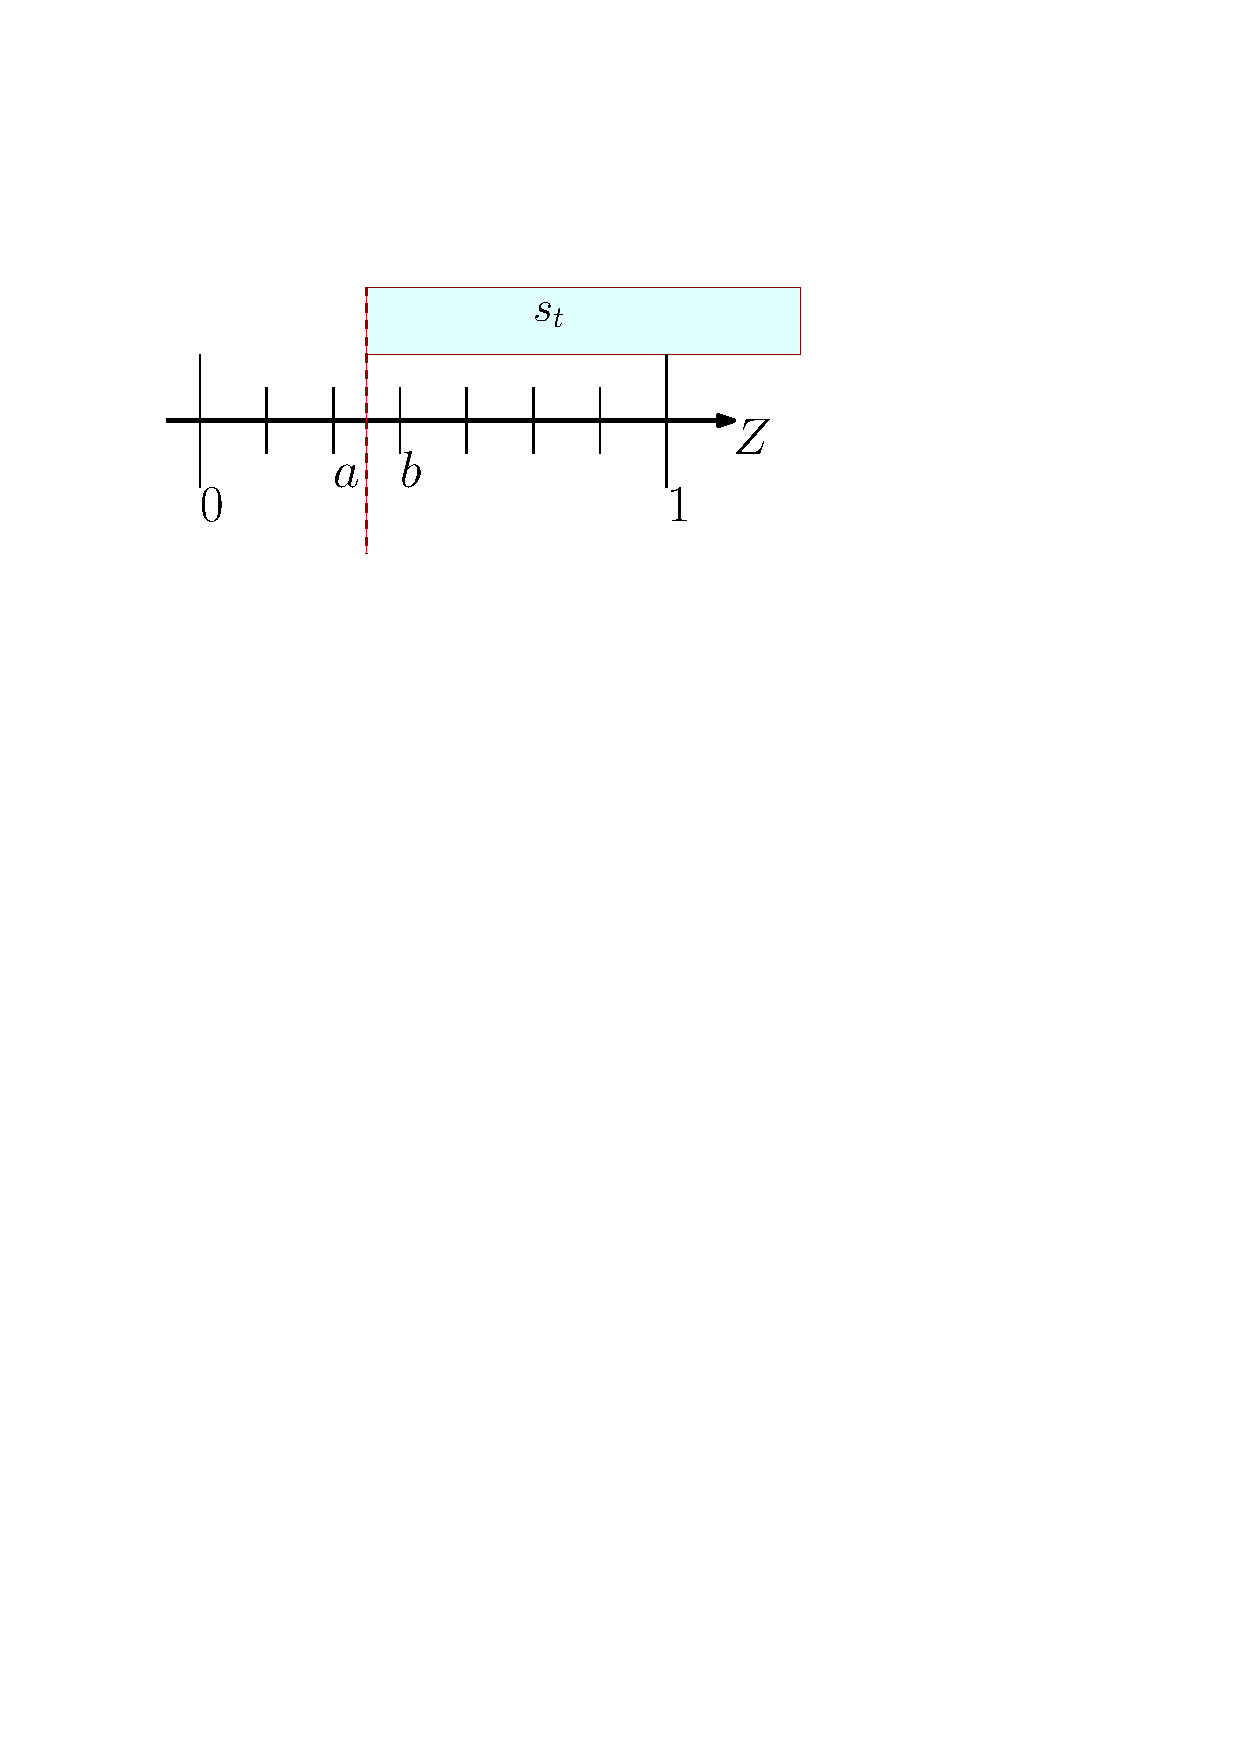
\includegraphics[width=0.22\textwidth]{images/lemma2}
\caption{Sampling $t$ and the corresponding $S_t$}
\label{fig.lemma2}
\end{wrapfigure}

With $\V{z} \geq \V{0}$, scale $\V{z}$ \underline{s.t.} $\max(\V{z})=1$. This scaling is acceptable because the claim depends on ratios with $\V{z}$ and not the absolute values. Now, sample a threshold $t \in [0,1]$ using the probability density function $f(t) = 2t$. Note that $\pr[t \in [a,b]] = \int_{a}^{b}f(t) dt = b^2 - a^2$. This distribution is picked as a proof trick and does not affect the outcome of Cheeger's inequality. 

Define $S_t = \{v:\V{z}(v)>t\}$. So, picking $S_t$ depends on $t$ discretely. If $t$ is between $a$ \& $b$, then $\pr[v \in S_t] = b^2 - a^2$. This selection of $S_t$ is shown in Figure \ref{fig.lemma2}. Next, the denominator of Lemma \ref{lem2}
\begin{align*}
\mathbb{E}_t[\vol(S_t)] &= \mathbb{E}_t\bigg[\sum_v\mathrm{deg}(v)\mathbbm{1}[v\in S_t]\bigg], \\
&= \sum_v \mathrm{deg}(v) \underbrace{\mathbb{E}_t[\mathbbm{1}[v\in S_t]]}_{\parbox{6.5em}{\raggedright\scriptsize$\pr[v \in S_t] =\pr[t \in [0,\V{z}(v)]] =\V{z}(v)^2$}}, \\
&= \sum_v \mathrm{deg}(v) \V{z}(v)^2 \\
&= \V{z}^{\top}\V{D}\V{z}.
\end{align*}

For the numerator,
\begin{align*}
\mathbb{E}_t[\abs{E(S,\overline{S})}] &= \mathbb{E}_t\bigg[\sum_{(u,v)}\mathbbm{1}[(u,v)\in E(S_t,\overline{S_t})]\bigg] \\
&= \sum_{(u,v)}\pr[(u,v) \in E(S_t,\overline{S_t})] \\
&= \sum_{(u,v)}\abs{\V{z}(u)^2-\V{z}(v)^2}.
\end{align*}

Applying Cauchy-Shwartz inequality $\bigg( \sum_ia_ib_i \leq \sqrt{\sum_ia_i^2} \sqrt{\sum_ib_i^2} \bigg)$ gives
\begin{align*}
\sum_{(u,v)}\abs{\V{z}(u)^2-\V{z}(v)^2} &\leq \sqrt{(\underbrace{\sum_{(u,v)}(\V{z}(u)-\V{z}(v))^2}_{\footnotesize \text{Laplacian quadratic form}})(\sum_{(u,v)}(\V{z}(u)+\V{z}(v))^2)}, \\
\sum_{(u,v)}(\V{z}(u)+\V{z}(v))^2 &\leq 2\sum_{(u,v)}(\V{z}(u)^2+\V{z}(v)^2) \\
&= 2\sum_v\text{deg}(v)\V{z}(v)^2 \\
&= 2\V{z}^{\top}\V{D}\V{z}.
\end{align*}
Therefore,
\begin{equation*}
\dfrac{\mathbb{E}_t[\abs{E(S,\overline{S})}]}{\mathbb{E}_t[\vol(S_t)]} \leq \dfrac{\sqrt{2(\V{z}^{\top}\V{L}\V{z})(\V{z}^{\top}\V{D}\V{z})}}{\V{z}^{\top}\V{D}\V{z}} = \sqrt{\ 2\ \dfrac{\V{z}^{\top}\V{L}\V{z}}{\V{z}^{\top}\V{D}\V{z}}}
\end{equation*}

%Proof of Lemma 3
\subsection{Lemma \ref{lem3}} \label{sec.lem3}
Assuming the collection of $X_t, Y_t$ is finite, let $r$ denote the
minimum ratio, and without loss of generality, assume that it is
achieved for $t=0.$
\begin{align*}
r & \defeq \min_t \dfrac{X_t}{Y_t} \qquad \text{\underline{s.t.}} \, Y_t>0, \\
&= \dfrac{X_0}{Y_0}.
\end{align*}

% \noindent We want to prove that
% \[\frac{X_0}{Y_0} = r \le \frac{\av_t[X_t]}{\av_t[Y_t]}.\]
% \noindent We assume to the contrary that $r > $ that $r < $

The fact that $r$ is a minimum means that for all $t,$ we
have $r \le \frac{X_t}{Y_t},$ and hence $ r Y_t \le X_t$ (since $Y_t >
0$). Taking
expectation over $t,$ we get that
\[r \av_t [Y_t] \le \av_t[X_t],\]
or equivalently,
\[r \le \frac{\av_t[X_t]}{\av_t[Y_t]}.\]
(Note that $Y_t > 0$ for all $t,$ and hence $\av_t[Y_t] > 0.$)
Since $r = \frac{X_0}{Y_0},$ this proves the claim.
% \begin{align*}
% \dfrac{X_t}{Y_t} &\geq r, \\
% X_t &\geq rY_t, \\
% \mathbb{E}_t[X_t] &\geq r\mathbb{E}_t[Y_t]
% \end{align*}

%Examples
\section{Examples}
Given a vector $\V{y}$, how do we get a `good' cut? Consider two examples that we have seen previously, a single edge between two vertices and a ring graph.

%example1
\subsection{Two Vertices Connected by an Edge}
We know that $\Phi(G)=1$. Using Cheeger's inequality, we first compute the second smallest eigenvalue of the normalized graph Laplacian. Drawing from the first lecture,
\begin{align*}
\nu_2 &= \lambda_2(\V{D}^{-1/2}\V{L}\V{D}^{-1/2})\\
&= \lambda_2(\V{L}) \\
&= 2 \\
&= 2\Phi(G),
\end{align*}
showing that the lower bound of Cheeger's inequality is tight

%example2
\subsection{Ring Graph}

\begin{lemma}
For $R_n$, define
\begin{align*}
x_k(v) &= \sin(\frac{2\pi kv}{n}), \quad 0 \leq k \leq \frac{n}{2}, \quad \mathrm{and} \\
y_k(v) &= \cos(\frac{2\pi kv}{n}), \quad 0 \leq k \leq \frac{n}{2}.
\end{align*}
$\forall k$, $x_k, y_k$ are eigenvectors of $L_{R_n}$, with eigenvalues $2(1-\cos(\frac{2\pi k}{n}))$.
\end{lemma}

Proof of the above lemma is left as an exercise.

For the simple case of $n$ even,
\begin{equation*}
\Phi(R_n) = \dfrac{2}{2.\frac{n}{2}} = \dfrac{2}{n}
\end{equation*}

Knowing that $\V{D}=2\V{I}$,
\begin{align*}
\nu_2 &= \lambda_2(\V{D}^{-1/2}\V{L}\V{D}^{-1/2}) \\
&= \frac{1}{2}\lambda_2(\V{L}) \\
&= \frac{1}{2} (2-2\cos (\dfrac{2\pi}{n})) \\
&= 2 \sin^2(\dfrac{\pi}{n}) \\
&= 2 (\dfrac{\pi}{n})^2(1+o(1)), \quad \text{for large $n$}.
\end{align*}
Note that for a tight bound, we would need to take the square root of the above expression, as proven earlier. 

As an exercise, try finding graph cuts using Julia. Use the previous lecture's formulation and then use Cheeger's inequality to make cuts.

\newpage
\section{Random Walks}
%Random walk graph
\begin{wrapfigure}{r}{0.20\textwidth}
\centering
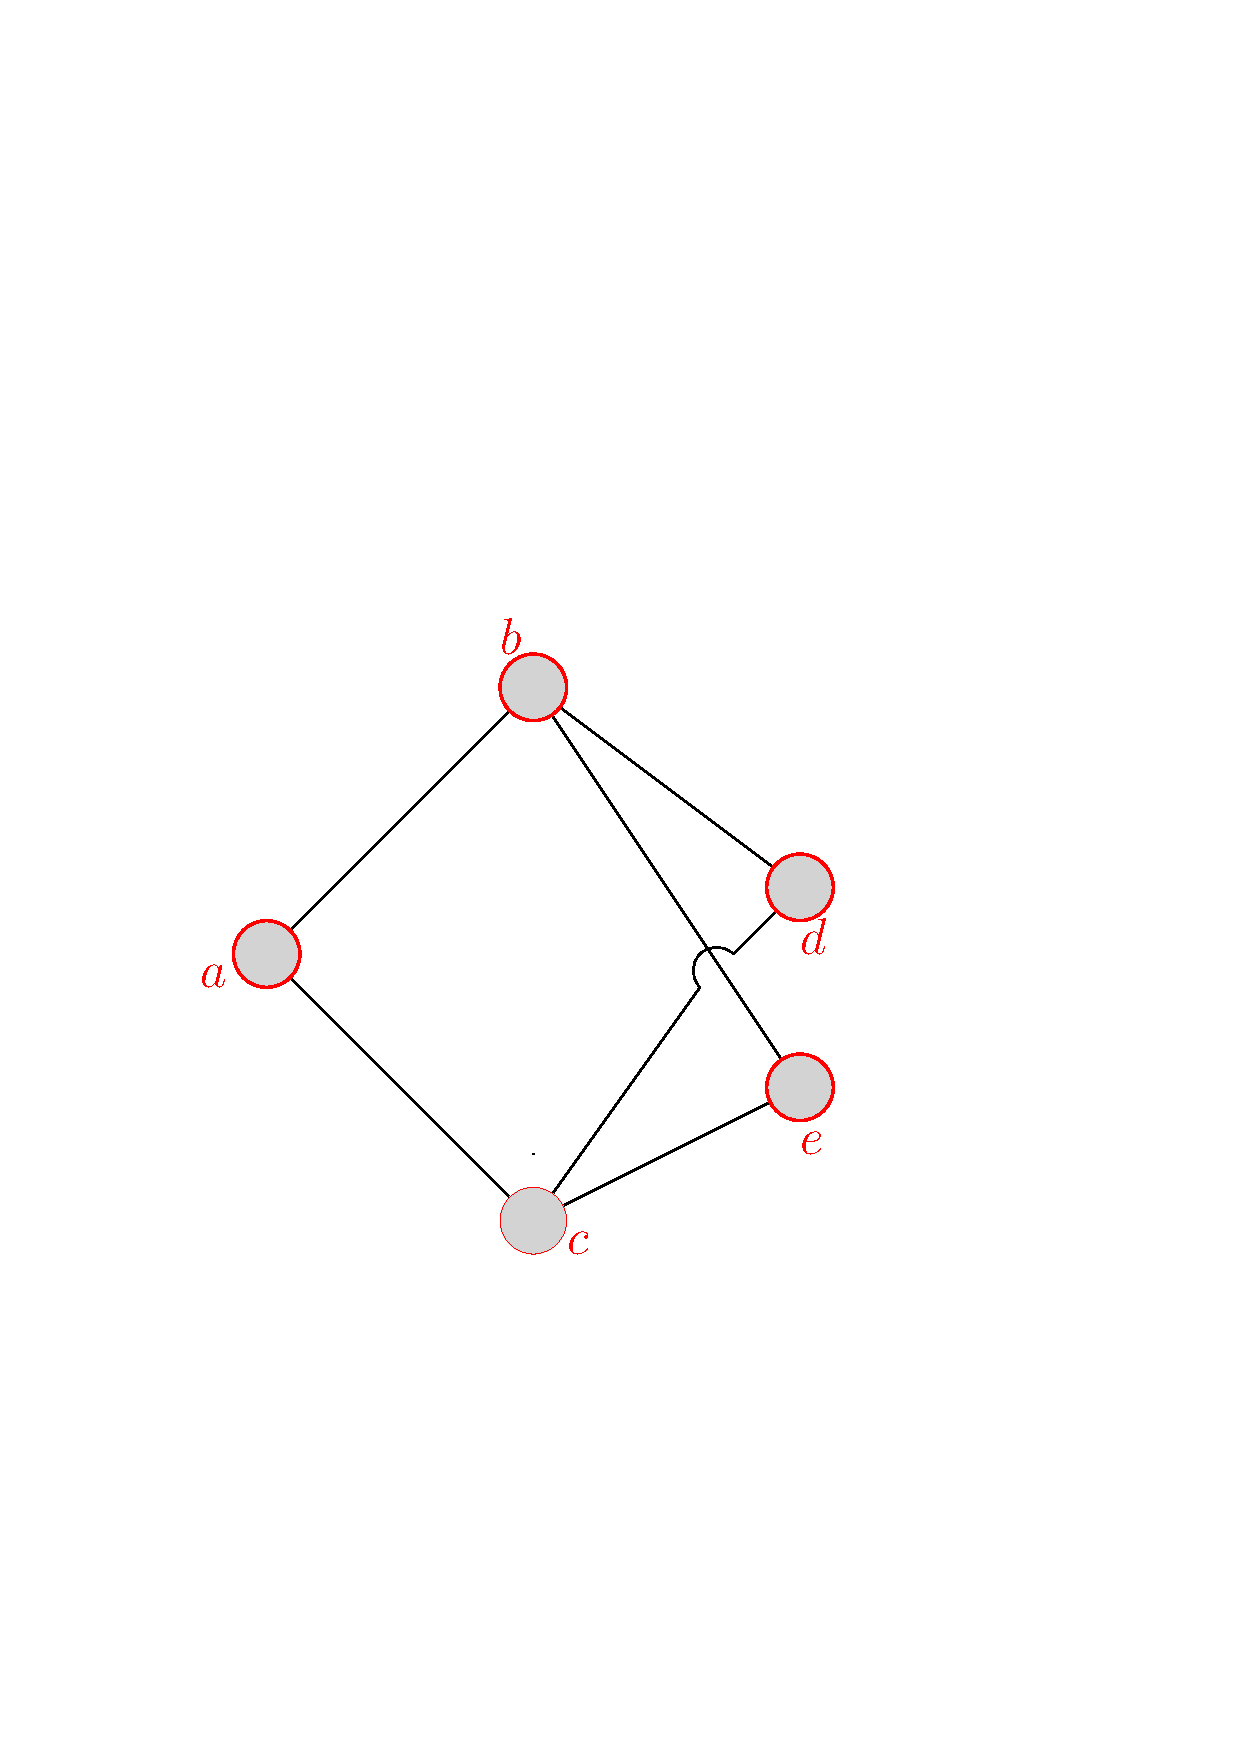
\includegraphics[width=0.20\textwidth]{images/randomwalk}
\caption{Example of random walk graph}
\label{fig.randomwalk}
\end{wrapfigure}

We will now be looking at undirected graphs that capture reversible Markov chains. Consider the graph in Figure \ref{fig.randomwalk}. Start with a peg on vertex $a$ at time $0$. Then, at time $1$, pick uniformly between neighbours to move to; in this case, $\pr[\text{$v=b$ at $t=1 \ |\ v=a$ at $t=0$}] = \pr[\text{$v=c$ at $t=1 \ |\ v=a$ at $t=0$}] = 0.5$. If the graph is weighted, scale the transition probabilities using the weights. The resulting sequence of vertices that have been visited over time is called the transcript of the random walk.

Given a graph and initial vertex, we are interested in answering questions such as,
\begin{itemize}
\item What is the distribution over vertices after a given number of steps?
\item Is there a stationary distribution?
\item How quickly do we converge?
\end{itemize}

The state evolution can be quantified using knowledge of the graph structure. At time $t$, define $\V{p}_t \in \mathbb{R}^V, \V{p}_t \geq \V{0},$ and $\mathbbm{1}^{\top}\V{p}_t = \sum_\V{v}\V{p}_t(v)=1$; let
\begin{align*}
\V{p}_0(v) &= \begin{cases}1 \quad &\text{if} \,\,\, v=a\\0 &\text{else}\end{cases} \quad \text{(starting at a)}, \\
\V{p}_t(v) &= \pr[\text{the random walk is at vertex $v$ at time $t$}], \\
\V{p}_{t+1}(v) &= \sum_{u:(u,v)} \dfrac{1}{\text{deg}(u)}\V{p}_t(u) \quad \text{(unweighted)}.
\end{align*}

For weighted graphs, deriving the following is left as an exercise:
\begin{align*}
\pr[\text{$v$ at $t+1$ $|$ $u$ at $t$}] &= \dfrac{w(u,v)}{\sum_{z:(u,z)}w(u,z)} = \dfrac{w(u,v)}{\underbrace{\text{deg}(u)}_{\footnotesize\text{weighted deg}}}, \\
\V{p}_{t+1}(v) &= \sum_{u:(u,v)} \dfrac{w(u,v)}{\text{deg}(u)}\V{p}_t(u), \\
\V{p}_{t+1} &= \V{A}\V{D}^{-1}\V{p}_t.
\end{align*}

\end{document}


%%% Local Variables:
%%% mode: latex
%%% TeX-master: t
%%% End:
